% 
%            ,,                                        
%          `7MM            _.o9                                
%            MM                                             
%  ,6"Yb.    MM  ,p6"bo   ,6"Yb.  M"""MMV  ,6"Yb.  `7Mb,od8 
% 8)   MM    MM 6M'  OO  8)   MM  '  AMV  8)   MM    MM' "' 
%  ,pm9MM    MM 8M        ,pm9MM    AMV    ,pm9MM    MM     
% 8M   MM    MM YM.    , 8M   MM   AMV  , 8M   MM    MM     
% `Moo9^Yo..JMML.YMbmd'  `Moo9^Yo.AMMmmmM `Moo9^Yo..JMML.   
% 
% 
% Free and Open-Source template for academic works
% https://github.com/dpmj/alca



\subsection{Kubeflow}

Kubeflow è un framework open-source e comunitario progettato per semplificare il ciclo di vita completo delle applicazioni di machine learning su Kubernetes. Offre una suite completa di strumenti e risorse per l'implementazione, l'orchestrazione e la gestione di workflow di machine learning su infrastrutture Kubernetes. Questo ecosistema avanzato consente agli sviluppatori e agli ingegneri di dati di sfruttare le potenzialità delle moderne architetture distribuite per la costruzione di modelli di machine learning scalabili e gestibili.

\begin{figure}[h]
    \centering
    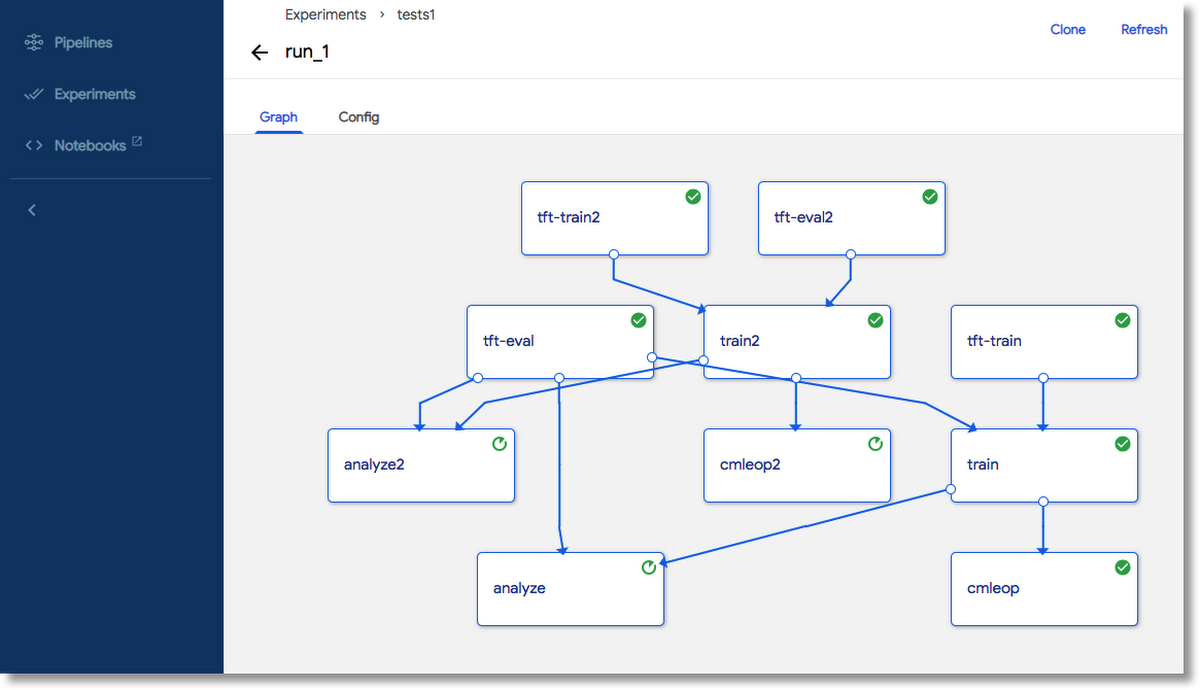
\includegraphics[width=\linewidth]{figures/ch3/kubeflow-ui.png}
    \caption[Interfaccia utente di una pipeline di Kubeflow]{Interfaccia utente di una pipeline di Kubeflow}
    \label{fig:cha3:kf-arch}
\end{figure}

\subsubsection{Architettura di Kubeflow}

L'architettura di Kubeflow è strutturata per fornire un ambiente coeso per lo sviluppo e la distribuzione di modelli di machine learning. Alcuni dei componenti chiave includono:

\begin{itemize}
    \item \textbf{Katib (Optimizator)}: E' un componente di Kubeflow dedicato all'ottimizzazione degli iperparametri. Basato su algoritmi di ricerca automatica, come Bayesian Optimization, Katib facilita il tuning degli iperparametri dei modelli di machine learning in modo efficiente e automatizzato.

    \item \textbf{KFServing}: Si occupa della distribuzione dei modelli di machine learning come servizi scalabili e gestibili. Supporta diversi framework di machine learning, consentendo la distribuzione in modo uniforme e il routing del traffico tra le diverse versioni del modello.

    \item \textbf{PyTorch Operator e TensorFlow Operator}: Gli operatori specifici per PyTorch e TensorFlow semplificano l'esecuzione di workload di machine learning basati su questi framework su Kubernetes. Gli operatori semplificano la creazione, l'aggiornamento e la gestione dei modelli, garantendo una maggiore facilità d'uso.

    \item \textbf{Kubeflow Pipelines}: Fornisce uno strumento per definire e orchestrare flussi di lavoro di machine learning complessi. Basato su Tekton, Kubeflow Pipelines permette la creazione di pipeline che integrano passaggi di addestramento, valutazione e distribuzione di modelli.

    \item \textbf{Kubeflow Katib Service}: Questo servizio offre un'API per l'interazione con Katib, consentendo agli utenti di definire esperimenti di ottimizzazione degli iperparametri e monitorarne i risultati.

    \item \textbf{Kubeflow Central Dashboard}: La dashboard centrale di Kubeflow fornisce un'interfaccia grafica per la gestione e il monitoraggio delle risorse di machine learning su Kubernetes. Integra viste specifiche per le diverse fasi del ciclo di vita di un modello, semplificando il controllo e la gestione complessiva.
\end{itemize}

\begin{figure}[h]
    \centering
    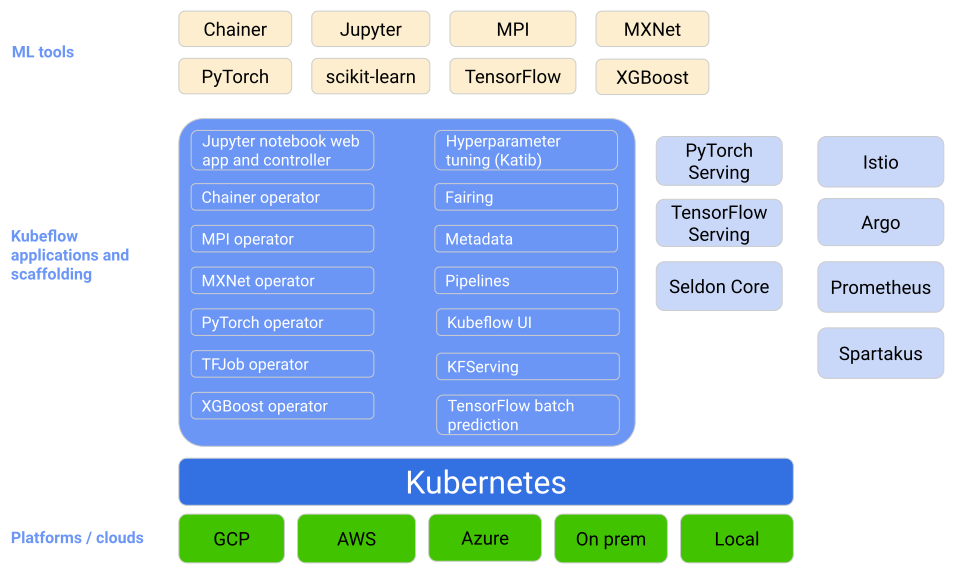
\includegraphics[width=\linewidth]{figures/ch3/kubeflow-arch.png}
    \caption[Architettura di un cluster Kubeflow]{Architettura di un cluster Kubeflow}
    \label{fig:cha3:kf-arch}
\end{figure}

L'efficacia di Kubeflow risiede nella sua capacità di integrare nativamente le best practices di Kubernetes nel contesto del machine learning. L'utilizzo di operatori specifici per framework di machine learning, la gestione degli esperimenti di ottimizzazione degli iperparametri e la distribuzione dei modelli come servizi sono solo alcune delle caratteristiche distintive che sottolineano l'approccio avanzato di Kubeflow al machine learning su Kubernetes.

\subsubsection{Sviluppo dei componenti}

Lo sviluppo di componenti personalizzati all'interno di Kubeflow risponde alla necessità di adattare l'ecosistema alle esigenze specifiche di un'applicazione di machine learning o di un processo lavorativo particolare. Questo approccio permette agli sviluppatori di estendere le funzionalità di Kubeflow in modo modulare, affrontando sfide specifiche e migliorando l'integrazione con il flusso di lavoro di machine learning.

Sviluppare componenti personalizzati in Kubeflow offre un livello di flessibilità senza pari. Questi componenti possono essere progettati per adattarsi a requisiti aziendali unici, integrare con sistemi esistenti o automatizzare specifiche fasi del ciclo di vita del machine learning. Inoltre, la creazione di operatori personalizzati consente di semplificare la gestione delle risorse specifiche, fornendo un'astrazione ad alto livello per operazioni complesse.

La modularità dei componenti personalizzati consente agli sviluppatori di concentrarsi su un singolo aspetto senza compromettere l'integrità del sistema. Questi componenti possono essere riutilizzati in diversi contesti, facilitando la standardizzazione di processi e operazioni all'interno di un'organizzazione. Inoltre, contribuendo a un approccio di sviluppo guidato dalla comunità, gli sviluppatori possono collaborare per migliorare e arricchire il panorama di Kubeflow, garantendo una maggiore adattabilità e versatilità nel tempo.

Per fornire un esempio di sviluppo di un componente Kubeflow, esamineremo l'implementazione di un operatore personalizzato specifico per Kubeflow. Gli operatori personalizzati sono una parte essenziale di Kubeflow e semplificano la gestione di risorse specifiche all'interno di un cluster Kubernetes. Per questo esempio, supponiamo di voler creare un operatore personalizzato per gestire la registrazione e il monitoraggio degli esperimenti di machine learning su Kubeflow.

\begin{code}
\captionof{listing}{Fusion Classifier sub-pipeline}
\label{code:apx:a:python}
\begin{minted}{python}
from kubernetes import client, config
from kubernetes.client.rest import ApiException

class KubeflowExperimentOperator:
    def __init__(self, experiment_name):
        config.load_kube_config()
        self.experiment_name = experiment_name
        self.api_instance = client.CustomObjectsApi()

    def create_experiment(self):
        body = {
            "apiVersion": "kubeflow.org/v1alpha3",
            "kind": "Experiment",
            "metadata": {"name": self.experiment_name},
            "spec": {"objective": "MAXIMIZE", "algorithm": {"algorithmName": "random"}}
        }

        try:
            api_response = self.api_instance.create_cluster_custom_object(
                group="kubeflow.org",
                version="v1alpha3",
                plural="experiments",
                body=body,
            )
            print("Experiment created. Status='%s'" % str(api_response.status))
        except ApiException as e:
            return e

    def get_experiment_status(self):
        try:
            api_response = self.api_instance.get_cluster_custom_object_status(
                group="kubeflow.org",
                version="v1alpha3",
                plural="experiments",
                name=self.experiment_name,
            )
            return api_response["status"]
        except ApiException as e:
            return e
\end{minted}
\end{code}

\begin{code}
\captionof{listing}{Utilizzo del componente Kubeflow}
\label{code:apx:a:python}
\begin{minted}{python}
from kubeflow_experiment_operator import KubeflowExperimentOperator

# Creazione di un'istanza dell'operatore per l'esperimento "my_experiment"
operator = KubeflowExperimentOperator(experiment_name="my_experiment")

# Creazione di un nuovo esperimento
operator.create_experiment()

# Ottenimento dello stato dell'esperimento
experiment_status = operator.get_experiment_status()
print(f"Status of experiment: {experiment_status}")


\end{minted}
\end{code}

In questo esempio semplificato, l'operatore personalizzato {\small \verb|KubeflowExperimentOperator|} è progettato per creare e monitorare esperimenti di machine learning su Kubeflow. Utilizza la libreria kubernetes per interagire con l'API di Kubernetes, consentendo la creazione di risorse personalizzate come gli esperimenti.

Questa è solo un'implementazione basilare a scopo illustrativo. In una situazione del mondo reale, l'operatore personalizzato potrebbe includere funzionalità più avanzate, come la gestione delle risorse associate agli esperimenti o l'integrazione con altri componenti di Kubeflow.

\subsubsection{Progettazione di una pipeline di Machine Learning}

Immaginiamo di dover creare una pipeline Kubeflow che coinvolga diverse fasi di un tipico flusso di lavoro di machine learning, come l'addestramento di un modello, la valutazione e la distribuzione di un servizio di inferenza. 

In questa pipeline, utilizzeremo gli strumenti di Kubeflow Pipelines per definire e orchestrare queste fasi.

\begin{code}
\captionof{listing}{Creazione di una pipeline Kubeflow}
\label{code:apx:a:python}
\begin{minted}{python}
import kfp
from kfp import dsl
from kfp.components import func_to_container_op, InputPath, OutputPath
    
# Componenti personalizzati come funzioni Python
@func_to_container_op
def train_model(input_data: InputPath(), output_model: OutputPath()):
    # Codice per l'addestramento del modello
    # Salva il modello in output_model
    pass
    
@func_to_container_op
def evaluate_model(input_model: InputPath(), input_data: InputPath(), output_metrics: OutputPath()):
    # Codice per la valutazione del modello
    # Salva le metriche in output_metrics
    pass
    
    @func_to_container_op
    def deploy_model(input_model: InputPath(), serving_image: str):
    # Codice per la distribuzione del modello come servizio
    pass
    
# Definizione della pipeline
@dsl.pipeline(
    name="Machine Learning Pipeline",
    description="Una semplice pipeline di Machine Learning"
)

def ml_pipeline(data_path: str, serving_image: str):
    # Fase 1: Addestramento del Modello
    training_task = train_model(data_path, "/mnt/model")
    
    # Fase 2: Valutazione del Modello
    evaluation_task = evaluate_model(training_task.output, data_path, "/mnt/metrics")
    
    # Fase 3: Distribuzione del Modello
    deployment_task = deploy_model(evaluation_task.output, serving_image)
    
    # Compilazione e salvataggio della pipeline
    pipeline_func = ml_pipeline
    pipeline_filename = "ml_pipeline.yaml"
    kfp.compiler.Compiler().compile(pipeline_func, pipeline_filename)
\end{minted}
\end{code}
Ognuna delle funzioni rappresenta una fase specifica del nostro flusso di lavoro di machine learning. Successivamente, creiamo una pipeline Kubeflow utilizzando il decoratore {\small \verb|@dsl.pipeline|}. All'interno di questa pipeline, colleghiamo le fasi specificando gli output e gli input corrispondenti. Infine, compiliamo la pipeline utilizzando {\small \verb|kfp.compiler.Compiler|} e la salviamo in un file YAML.

\begin{figure}[h]
    \centering
    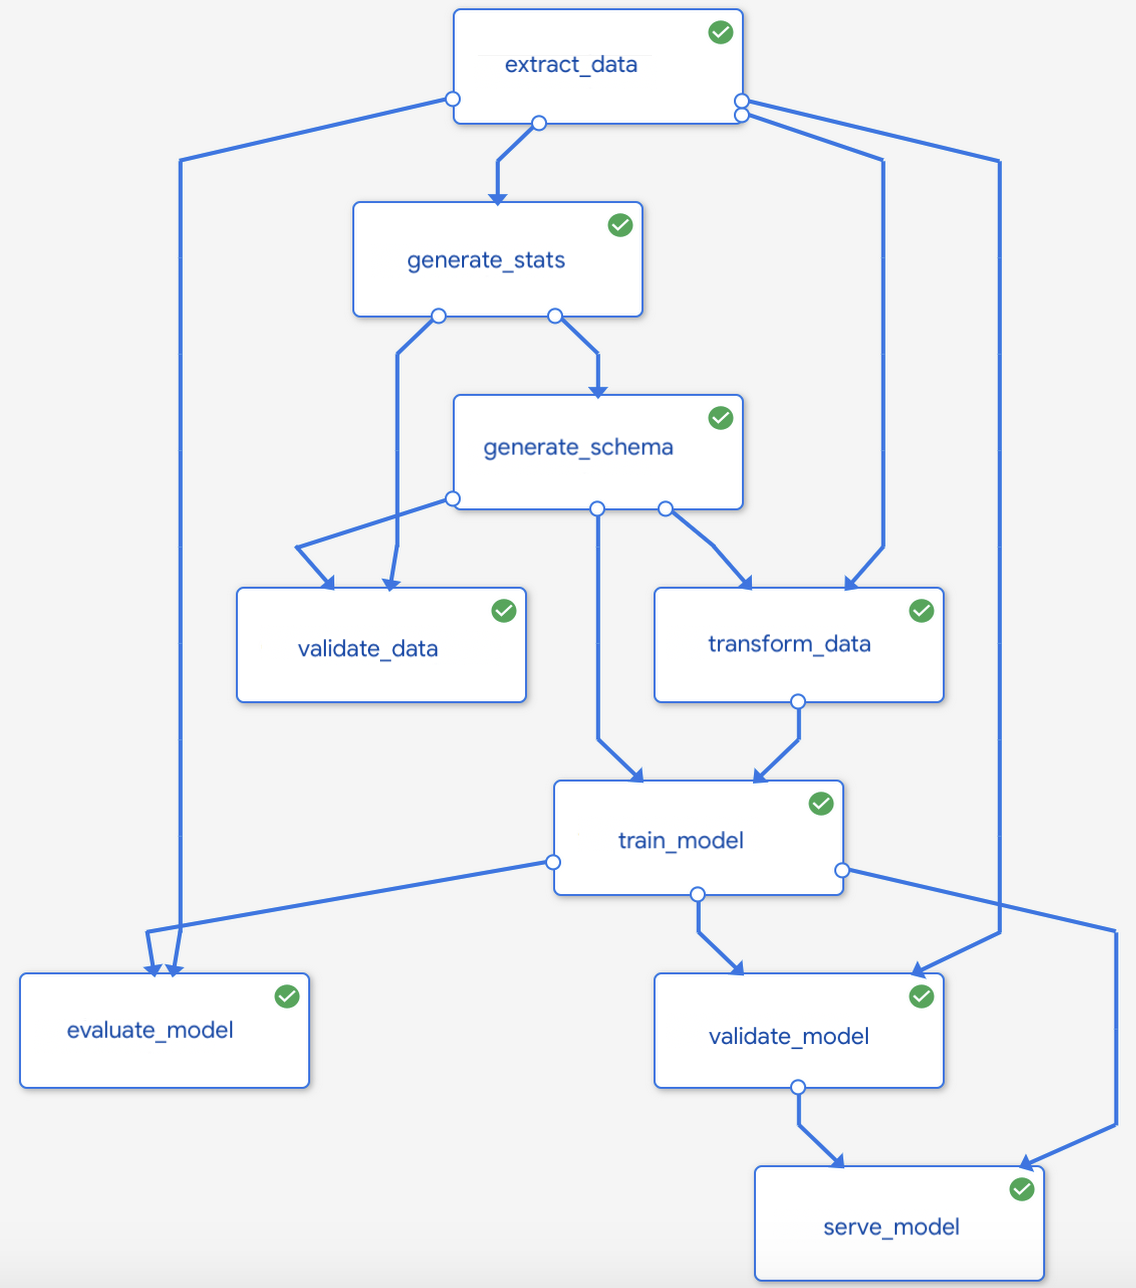
\includegraphics[width=350px]{figures/ch3/kubeflow-pipeline.png}
    \caption[Esempio di una pipeline Kubeflow]{Esempio di una pipeline Kubeflow}
    \label{fig:cha3:kf-pipe}
\end{figure}

Una volta che la pipeline è definita e compilata, può essere eseguita utilizzando l'interfaccia utente di Kubeflow o l'API di Kubeflow Pipelines.

Questo è un esempio semplificato e la pipeline può essere ulteriormente personalizzata in base alle esigenze specifiche del progetto, come l'aggiunta di passaggi di pre-elaborazione dei dati, l'ottimizzazione degli iperparametri o la gestione delle versioni dei modelli.

\subsubsection{Alternative a Kubeflow}

Naturalmente, Kubeflow non è l'unica piattaforma di sviluppo di pipeline di Machine Learning basata su Kubernetes. Esistono diverse alternative, come \glsname{mxnet}, \glsname{ray} ed \glsname{mlflow}.

La seguenti tabelle offrono una visione panoramica delle caratteristiche generali delle quattro tecnologie. 

\begin{table}[h]
    \centering
    \caption*{Orchestrazione}
    \begin{tabular}{|l|l|}
    \hline
    \textbf{Tecnologia} & \textbf{Piattaforma di Orchestrazione} \\ \hline
    Kubeflow & Kubernetes \\ \hline
    Ray & Proprio sistema di gestione delle risorse \\ \hline
    MXNet & Non specifico \\ \hline
    MLflow & Locale o in cloud \\ \hline
    \end{tabular}
    \end{table}
    
    \begin{table}[h]
    \centering
    \caption*{Supporto Framework ML}
    \begin{tabular}{|l|l|}
    \hline
    \textbf{Tecnologia} & \textbf{Framework ML Supportati} \\ \hline
    Kubeflow & Diversi \\ \hline
    Ray & Diversi \\ \hline
    MXNet & Solo MXNet \\ \hline
    MLflow & Diversi \\ \hline
    \end{tabular}
    \end{table}
    
    \begin{table}[h]
    \centering
    \caption*{Monitoring e Tracciabilità}
    \begin{tabular}{|l|l|}
    \hline
    \textbf{Tecnologia} & \textbf{Strumenti di Monitoring e Tracciabilità} \\ \hline
    Kubeflow & Integrazione nativa \\ \hline
    Ray & Strumenti specifici di Ray \\ \hline
    MXNet & Integrazione personalizzata \\ \hline
    MLflow & Logging integrato e tracciabilità \\ \hline
    \end{tabular}
    \end{table}

\clearpage